\begin{tikzpicture} [scale=0.9, transform shape]
	\onslide<1->{ \node[] (input_taj) 
		{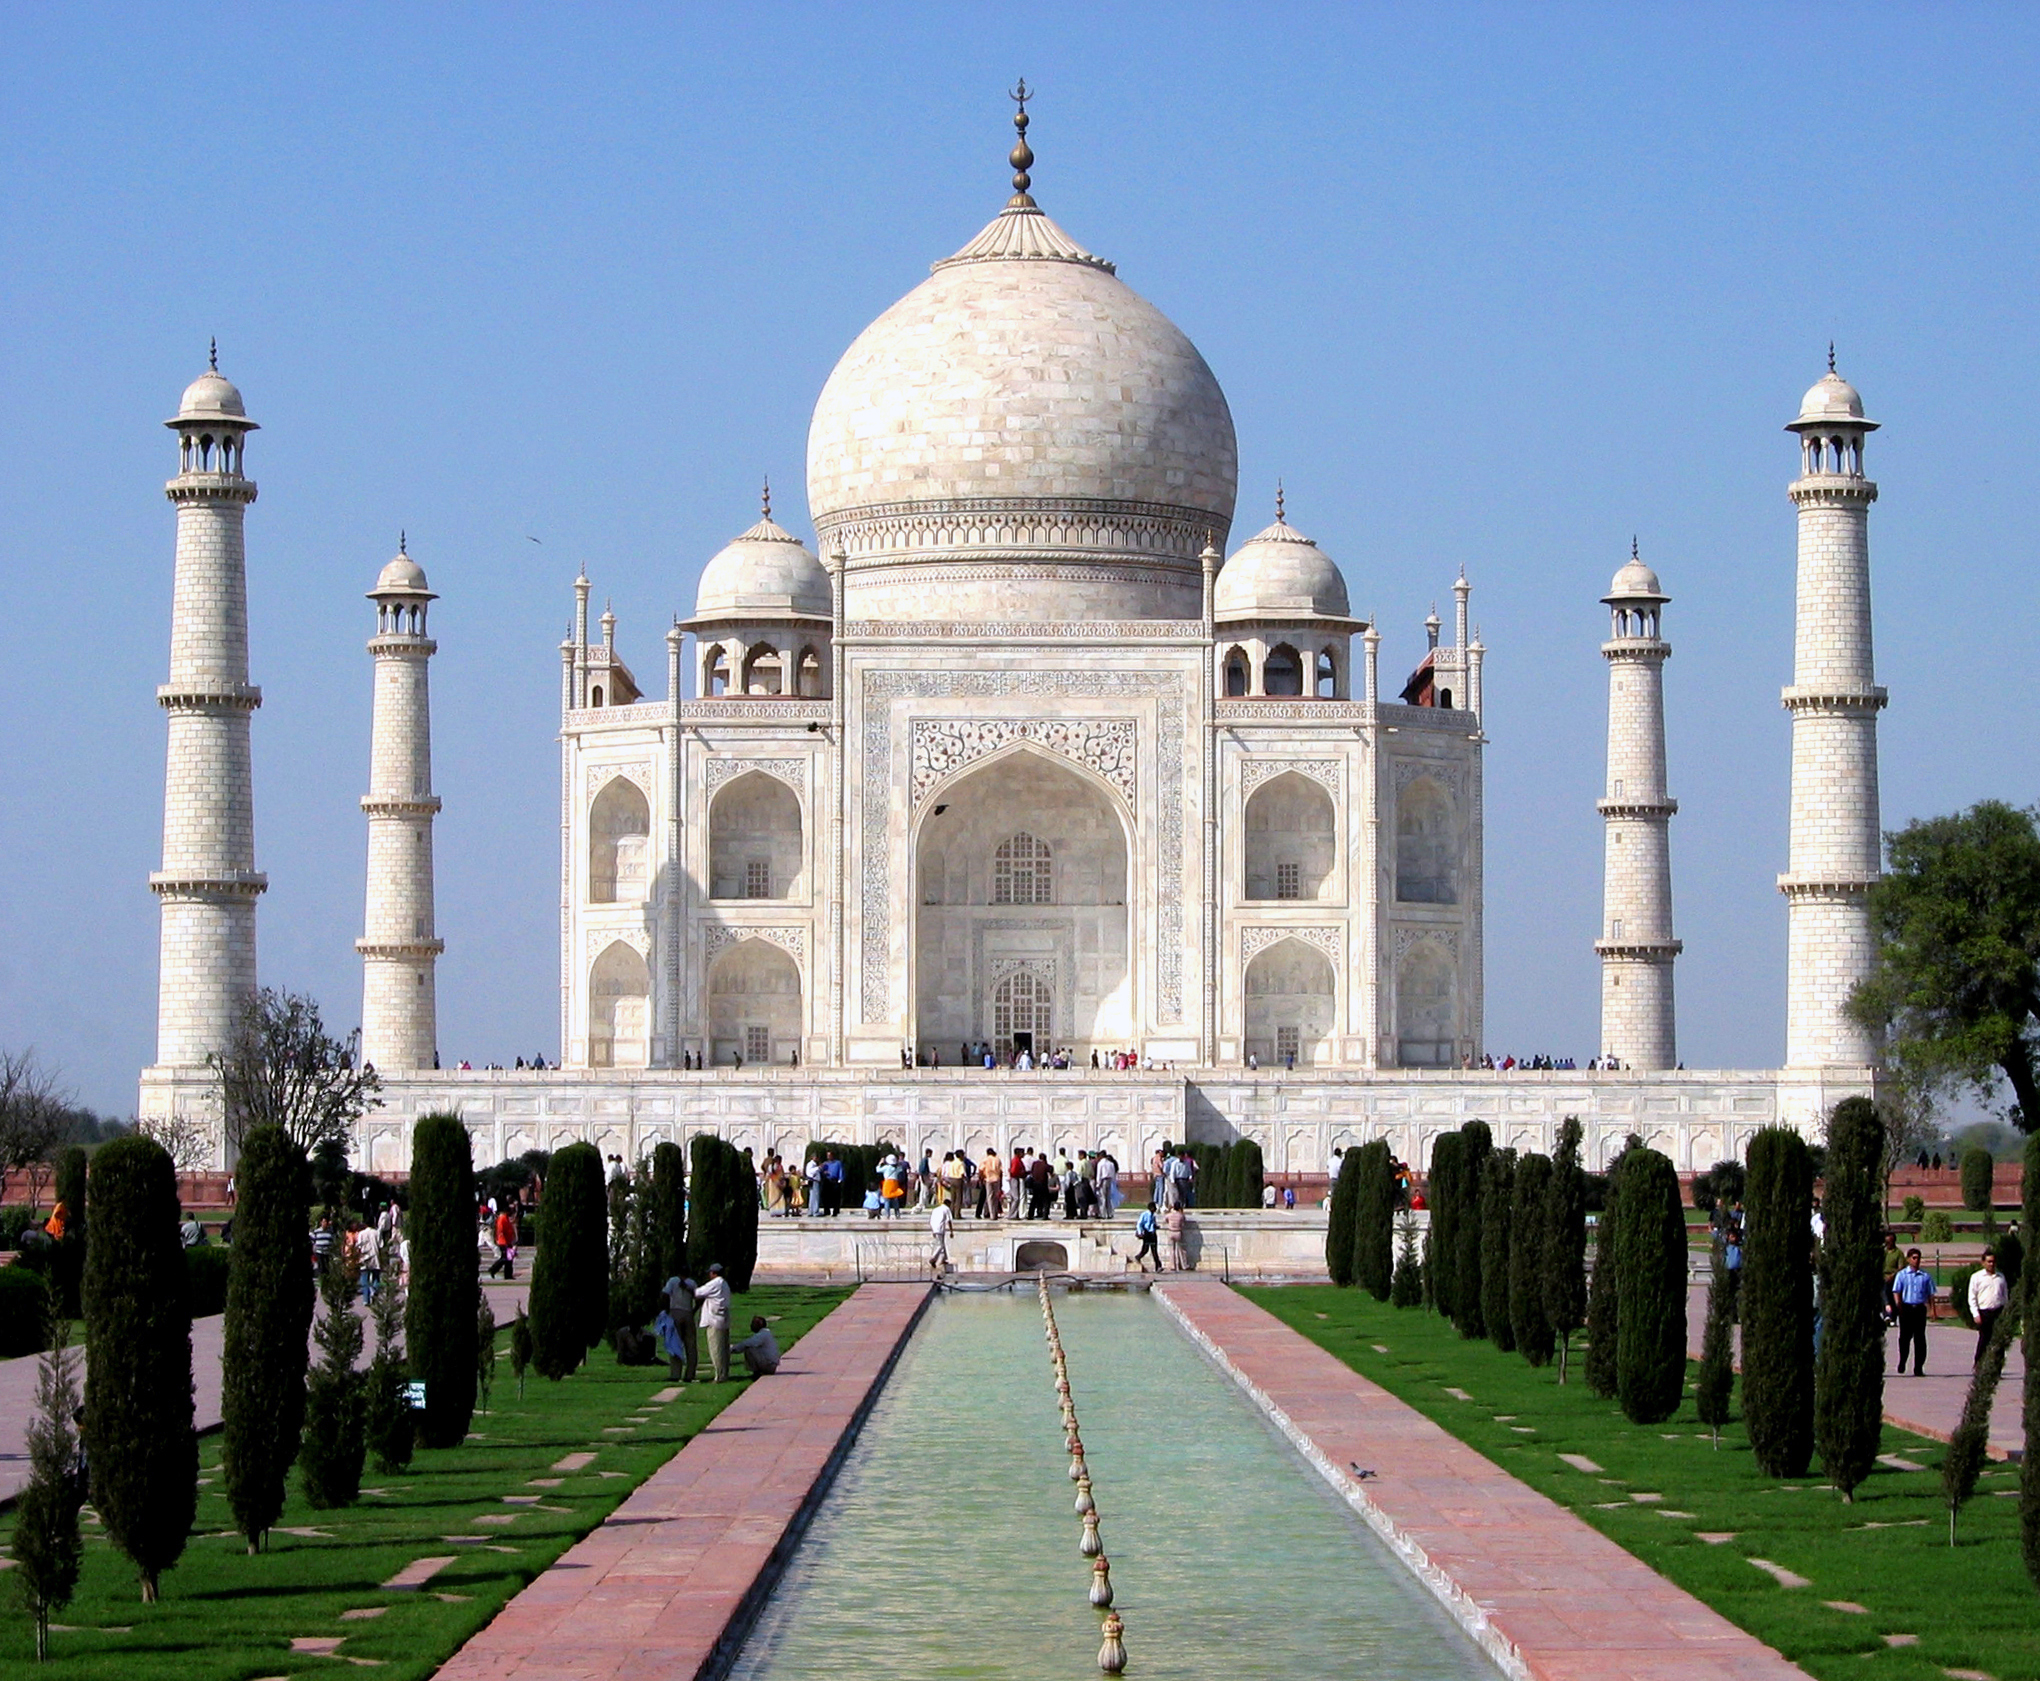
\includegraphics[width=20mm,height=17mm,scale=0.7]{images/taj_mahal.jpg}};
	}
	\onslide<1->{  \node (raw) at ($(input_taj) + (4, 0)$)  { 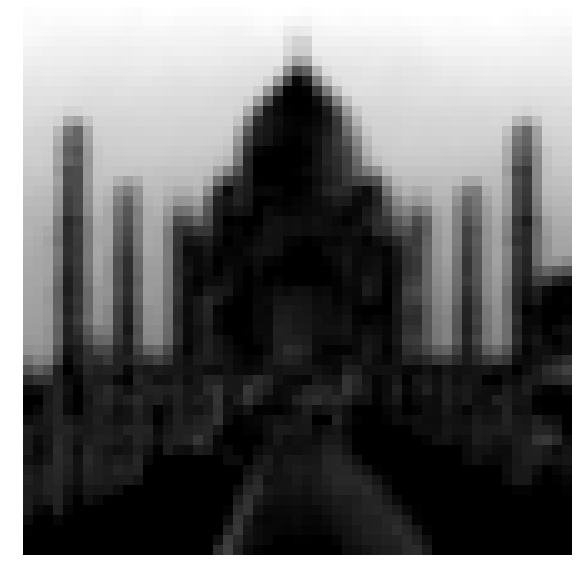
\includegraphics[width=20mm,height=17mm,scale=0.7]{images/convo1.png}};}
	\onslide<2->{\node (raw1) at ($(raw) + (0.2,0.2)$)  { 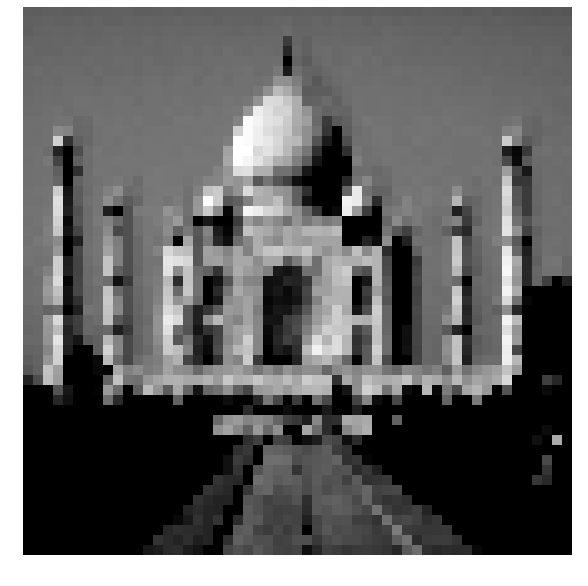
\includegraphics[width=20mm,height=17mm,scale=0.7]{images/convo1_49.png}};
	; }
	\onslide<3->{\node (raw2) at ($(raw1) + (0.2,0.2)$)  { 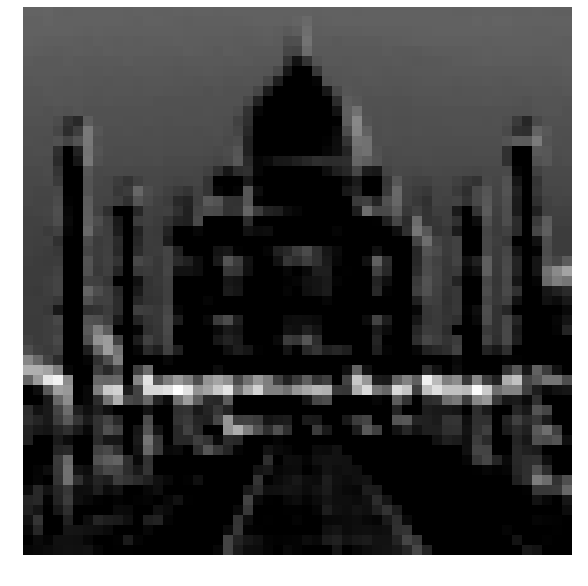
\includegraphics[width=20mm,height=17mm,scale=0.7]{images/convo1_74.png}}; }
	\onslide<1>{
		\node [below of = raw,anchor=north] (edge)  { \resizebox{25mm}{8mm}{ \begin{tabular}{ccccc}
			-1.21358689e-03  & 3.23652686e-03 & $\cdots$ & $\cdots$ & -2.06615720e-02\\ 
			-1.52757822e-03  & 2.36130832e-03 & $\cdots$ & $\cdots$ & -1.19824838e-02\\ 
			$\vdots$ & $\vdots$ &  &  & $\vdots$\\ 
			$\vdots$ & $\vdots$ &  &  & $\vdots$\\ 
			-8.25322699e-04 & -5.14897937e-03 &  $\cdots$ & $\cdots$ &-9.90395527e-03 \\
			\end{tabular} }};
		%\node[above of= raw,node distance=1.2cm ] (features)  {Features};
		\draw[->,thick] (input_taj) -- (raw) ;
	}
	\onslide<2>{ 
		\node [below of = raw,anchor=north] (edge)  { \resizebox{25mm}{8mm}{ \begin{tabular}{ccccc}
			-0.02337041 & -0.03243878 & $\cdots$ & $\cdots$ & -0.04728875\\ 
			-0.05375158 & -0.05350766 $\cdots$ & $\cdots$ & -0.04323674\\ 
			$\vdots$ & $\vdots$ &  &  & $\vdots$\\ 
			$\vdots$ & $\vdots$ &  &  & $\vdots$\\ 
			-0.00792501 & -0.00503319 &  $\cdots$ & $\cdots$ &0.00174674 \\
			\end{tabular} }};
		%\node[above of= raw,node distance=1.2cm ] (features)  {Features};
		\draw[->,thick] (input_taj) -- (raw) ;

	}
	\onslide<3->{
		\node [below of = raw,anchor=north] (edge)  { \resizebox{25mm}{8mm}{ \begin{tabular}{ccccc}
			-0.01871333 & -0.01075948 & $\cdots$ & $\cdots$ & 0.04684572\\ 
			0.00104325 & 0.01935937 & $\cdots$ & $\cdots$ & 0.01016542\\ 
			$\vdots$ & $\vdots$ &  &  & $\vdots$\\ 
			$\vdots$ & $\vdots$ &  &  & $\vdots$\\ 
			0.03008777 &  0.00335217 &  $\cdots$ & $\cdots$ &-0.02791128 \\
			\end{tabular} }};
		%\node[above of= raw,node distance=1.2cm ] (features)  {Features};
		\draw[->,thick] (input_taj) -- (raw) ;

	}
	\onslide<1->{\node [right=5cm of raw.center,anchor= center](output_taj){car, bus, \textcolor{blue}{monument}, flower};
		\draw[->,thick] (raw) -- (output_taj) ;}

\end{tikzpicture}